\documentclass{article}

\usepackage{pgf}
\usepackage{tikz}
\usetikzlibrary{arrows,automata}
\usepackage[latin1]{inputenc}
\begin{document}
\section{BuyOrder}
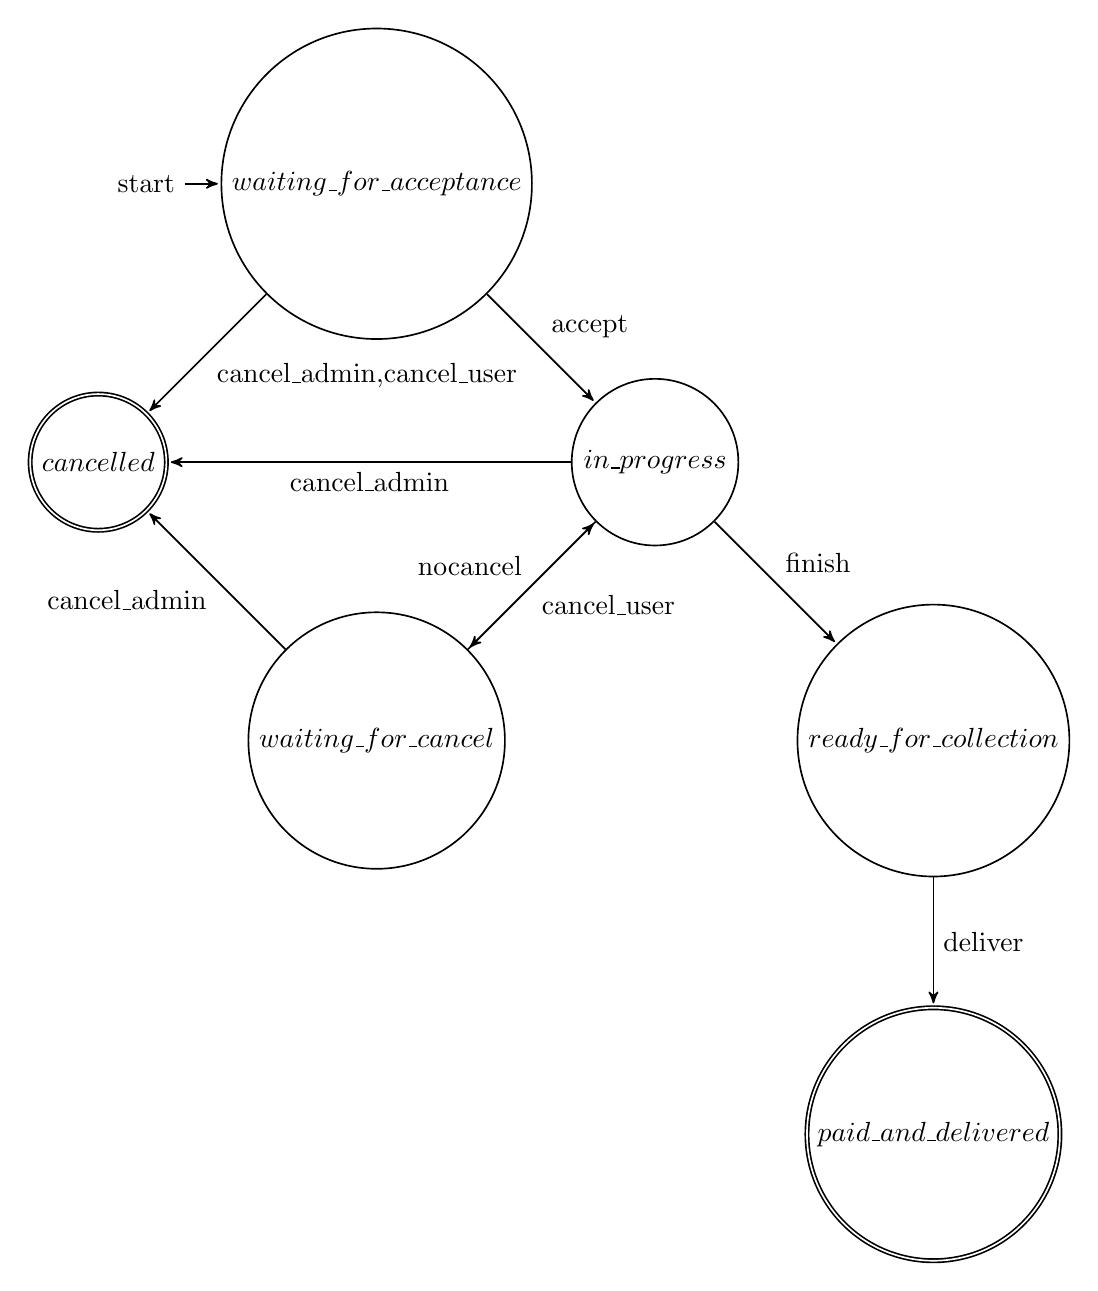
\begin{tikzpicture}[->,>=stealth',shorten >=1pt,auto,node distance=5cm,
                    semithick]
    \tikzstyle{every state}=[]

    \node[initial,state]  (A)                      {$waiting\_for\_acceptance$};
    \node[accepting,state](B) [below left of=A]    {$cancelled$};
    \node[state]          (C) [below right of=A]   {$in\_progress$};
    \node[state]          (D) [below left of=C]    {$waiting\_for\_cancel$};
    \node[state]          (E) [below right of=C]   {$ready\_for\_collection$};
    \node[accepting,state](F) [below of=E]         {$paid\_and\_delivered$};

    \path   (A) edge                node {cancel\_admin,cancel\_user} (B)
                edge                node {accept} (C)
            (C) edge                node {cancel\_admin} (B)
                edge                node {cancel\_user} (D)
                edge                node {finish} (E)
            (D) edge                node {cancel\_admin} (B)
            (D) edge                node {nocancel} (C)
            (E) edge                node {deliver} (F);
\end{tikzpicture}

\section{BorrowOrder}
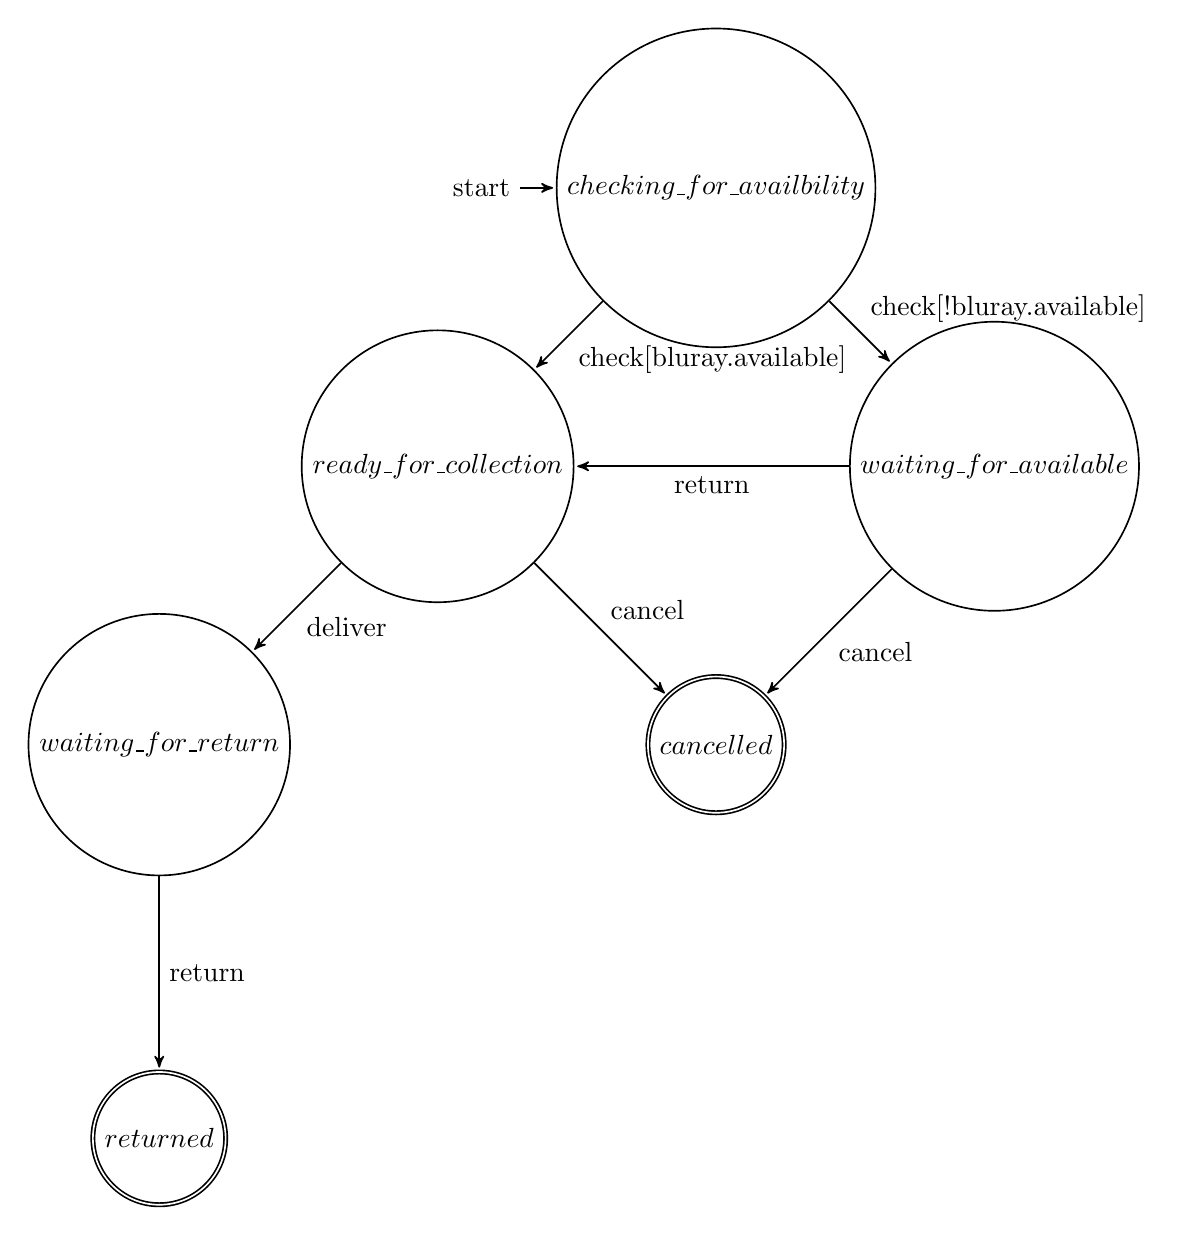
\begin{tikzpicture}[->,>=stealth',shorten >=1pt,auto,node distance=5cm,
                    semithick]
    \tikzstyle{every state}=[]

    \node[initial,state]  (A)                      {$checking\_for\_availbility$};
    \node[state]          (B) [below left of=A]    {$ready\_for\_collection$};
    \node[state]          (C) [below right of=A]   {$waiting\_for\_available$};
    \node[accepting,state](D) [below right of=B]    {$cancelled$};
    \node[state]          (E) [below left of=B]    {$waiting\_for\_return$};
    \node[accepting,state](F) [below of=E]         {$returned$};

    \path   (A) edge                node {check[bluray.available]}  (B)
                edge                node {check[!bluray.available]}  (C)
            (B) edge                node {cancel}                   (D)
                edge                node {deliver}             (E)
            (C) edge                node {cancel}                   (D)
                edge                node {return}             (B)
            (E) edge                node {return}                  (F);
\end{tikzpicture}

\end{document}
